%TEX TS-program = xelatex
\documentclass[11pt, twoside, openright]{book}
\usepackage[margin=2.54cm]{geometry} % set margins to 1 inch all the way around
\usepackage{fontspec}
	\defaultfontfeatures{Ligatures=TeX}
%	\newcommand{\lmr}{\fontfamily{lmr}\selectfont} % Latin Modern Roman
%	\setmainfont{Birka LT Pro}
	\setmainfont{Kepler Std Light}
	\setsansfont[Mapping=tex-text]{Myriad Pro}
	\setmonofont[Scale=MatchLowercase]{Anonymous Pro}
\usepackage{titlesec}
\titleformat{\chapter}[display]
    {\huge\bfseries\sffamily}{\chaptertitlename\ \thechapter}{20pt}{\Large}[\titlerule]
%this would be used to change section headings
%\titleformat{\section}{\Large\bfseries\sffamily}    
% set up indexing for all the acronyms
\usepackage{makeidx}
\makeindex
\usepackage[acronym,toc]{glossaries}
\makeglossaries
\usepackage{graphicx}   % this handles the non-native charts
\usepackage[sectionbib]{chapterbib} % this handles references per chapter
% this handles the risk equation -- may not be necessary
%\usepackage{amsmath}

%\usepackage[font=sf, labelfont={sf,bf}, margin=1cm]{caption}
\usepackage[font=small]{caption}
\PassOptionsToPackage{hyphens}{url}\usepackage{hyperref}
\renewcommand{\UrlBreaks}{\do\/\do\a\do\b\do\c\do\d\do\e\do\f\do\g\do\h\do\i\do\j\do\k\do\l\do\m\do\n\do\o\do\p\do\q\do\r\do\s\do\t\do\u\do\v\do\w\do\x\do\y\do\z\do\A\do\B\do\C\do\D\do\E\do\F\do\G\do\H\do\I\do\J\do\K\do\L\do\M\do\N\do\O\do\P\do\Q\do\R\do\S\do\T\do\U\do\V\do\W\do\X\do\Y\do\Z} % this handles breaking URLS smartly
\usepackage{enumitem}
\usepackage{setspace}
    \onehalfspacing % set line spacing to 1.5
    
%\newcommand\smallcaps[1]{{\footnotesize\textbf{#1}}}
\newcommand\climatedge{ClimatEdge\texttrademark{} }
\newcommand\ce{ClimatEdge 2.0 }

%\setlist{nolistsep}
\pagestyle{empty}
\setlength{\parindent}{0pt} % don't indent paragraphs globally

\begin{document}
	%!TEX root=index.tex
\begin{titlepage}
    \vspace*{\fill}
    \begin{center}
        \textbf{\Large Christopher Keller}\\[1cm]
        \textit{A Big Data Approach To ClimatEdge\texttrademark{}}\\ [.5cm]
        CSC NPS Solution Leadership Institute\\ [.5cm]
        %\today
        March 28, 2014
    \end{center}
    \vspace*{\fill}
\end{titlepage}

    \tableofcontents
	%!TEX root=index.tex

% establish that there is a business problem and the hypothesis should solve it
% maybe 1-1.5 pages
\newacronym{merra}{MERRA}{Modern-Era Retrospective analysis for Research and Applications}
\newacronym{html}{HTML}{Hyper Text Markup Language}
\newacronym{sme}{SME}{Subject Matter Expert}
\newacronym{pdf}{PDF}{Portable Document Format}
\chapter{Introduction}
\textsc{CSC's} \climatedge reports service offers the financial, utilities and agriculture risk industries a view into climate prediction based on proprietary analysis of public data. The monthly reports include Global Agriculture, Global Energy, Sugar and Soft Commodities, Grain and Oilseeds, and Energy/Natural Gas\cite{climatedgeurl}. The current method of generating these reports takes a high level cursory analysis and only analyzes a fraction of the data that is available. By applying \index{big data} storage and analytics technologies, I will show that \textsc{CSC} can quantitatively analyze more data and modernize the production of \climatedge reports. The resulting climate models will have greater confidence and be of more value to our customers.\\

\climatedge reports are based off knowledge acquired by programmatically parsing and summarizing the \gls{html} interface of the Giovanni\cite{giovanni} portal to the NASA \gls{merra} data site.  A \textsc{CSC} \gls{sme} then takes this data collection, adds analysis and annotations, and generates a \gls{pdf} report which details the risk potential thirty to sixty days in the future. In contrast, typical industry reports focus on seven to fourteen days in the future. There are a few drawbacks with this approach:
\begin{itemize}
    \item{limits the data acquisition to only that summary information that the Giovanni \index{Giovanni} maintainers choose to expose, rather than the raw data itself}
    \item{reports are generated per industry rather than per customer}
    \item{reports are resource intensive to produce}
\end{itemize}
I hypothesize that if \textsc{CSC} were to ingest the \gls{merra} archive, as well as other publicly available data sets, into a corporately managed data store with an analytical layer above, we could eliminate the dependency on NASA's Giovanni summary interface, as well as expanding the capabilities offered by \climatedge. By utilizing results based on analytics computed over the entire data set, we could add a quantitative probability to the existing qualitative analysis of \climatedge prediction reports. The technology, skills, and infrastructure used in the creation of the proprietary \gls{merra} solution, would be transferable to other big data projects within the company as a whole.\\


CNK -we need to say something here about prediction


Implementing a quantitative analysis component in a \ce service allows for several competitive advantages:
\begin{itemize}
    \item{the ingestion of additional datasets such as \textsc{ENSO}, \textsc{NAO/AO}, and \textsc{PDO}\cite[p. 1]{methods}}
    \item{the ability to organize the data on a per-solution basis, e.g., by time, by geographical location, etc}
    \item{the ability to scale the solution to the customer, e.g., faster reports cost more}
    \item{unique customer portals with the ability to generate reports on demand}
\end{itemize}
In conversations with Dr. Christopher Anderson and Dr. Dan Walker, I have identified three use cases in which a \ce service can benefit the risk insurance industry[personal communication, 2013]:
\begin{itemize}
    \item tornado prediction
    \item flood prediction
    \item commodities trading
\end{itemize}
By focusing on predictive analytics using large data sets we can use the following equation for the risk insurance industry:
\begin{equation*}
    Risk = Impact \cdot Probability
\end{equation*}
The current implementation of \climatedge can not address either of these variables.

%\begingroup
    % this removes the chapter title for the in-chapter bibliography
%    \renewcommand{\chapter}[2]{}% for other classes
\renewcommand\bibname{{References}}
\bibliographystyle{plain}
\bibliography{chapter1}
%\endgroup


	%!TEX root=index.tex

\newacronym{ncdc}{NCDC}{National Climatic Data Center}
\newacronym{soi}{SOI}{Southern Oscillation Index}
\newacronym{tvs}{TVS}{National Tornado Vortex Signature}
\newacronym{mda}{MDA}{National Mesoscyclone Detection Algorithm}

\chapter{Case Study}
\section*{Tornado}
A primary carrier of property and casualty insurance would potentially be very interested in knowing the probability of tornado occurrence in geographical areas in which they have a large customer base. There are two months in the year which kick off tornado season in the United States: the warm season starting in March, and the cold season starting in November. Having accurate predictions of weekly seasonal tornado counts months in advance, would constitute a significant business advantage over competitors. There are two specific business cases for the property carrier to focus on:
\begin{itemize}
    \item an actuary who will use the historical year-to-year probability and future counts to create overlays based on parcel level policy and claims data on a 50km x 50km geographical grid
    \item an underwriter who will use actuarial information to create the appropriate terms and rates offering for their customers that maximizes revenues at the lowest risk level
\end{itemize}
A working group, consisting of Dr. Christopher Anderson, Dr. Dan Walker, and myself, has determined that the data layer for tornado prediction should contain the following [unpublished, 2013]:
\begin{itemize}
    \item \gls{merra} 3D historical data set\cite{mdisc}
    \item \gls{soi} historical archives\cite{bom}
    \item \gls{tvs} and \gls{mda}\cite{hdss} 
    \item \gls{ncdc} historical tornado report\cite{ncdc}
\end{itemize}
All of this data is in the public domain and freely available to anyone that has the resources to store and analyze it. As mentioned in chapter one, currently CSC uses only the summary information provided by Giovanni in the \climatedge product. While Giovanni has the advantage of requiring no local computational resources, it represents the tip of the proverbial data iceberg and does not help in quantitative prediction.\\

Combinations of the data sets listed above can vary in size from a few hundred gigabytes to a few hundred terabytes just for the raw data. In order to quantitatively process this data, we need a service platform capable of performing the following operational layers:
\begin{itemize}
	\item retrieving data updates
	\item storing and indexing for optimal retrieval
	\item data discovery and analytics
	\item presenting real-time and offline results
\end{itemize}
\subsection*{Data Acquisition}
As all the data is freely available via standard HTTP requests, we simply need to put together a framework consisting of a repeatable process that polls each website for newly published data and retrieves it. If necessary, the framework can check with the data store to confirm what's new and what's not. Putting together such a framework is a relatively simple systems integration and development task and has plenty of prior art across the industry. I'd recommend the following components:
\begin{itemize}
	\item Three Linux instances to handle retrieval, monitoring, and hosting the source code repository, respectively.
	\item Jenkins for continually monitoring and notifying the success or failure of the retrieval processes (one per data set). Jenkins will also serve as the means to deploy the most recent code from the code repository onto the server handling the retrieval process. Jenkins is open source and used commonly across the industry for this purpose, resulting in an easily hirable skill set.\cite{jenkins}
	\item A repeatable method, such as Cron, to check and retrieve updated data sets at well defined publication intervals. Jenkins will monitor the success or failure of the cron jobs and notify as needed.
	\item Developed code that contacts each web server and pulls down only the most recent data. If the data sets do not offer a simple means of determining what's recent, this code can query the data store so that it's aware of the last stored data. While we need unique code for each data set, the process of determining what's new and retrieving the code should be very similar across all the data sets. It's likely there will a reusable common library of functionality across each specific implementation. This development is likely to be done in a scriptable environment such as Python or Perl. The languages offer an excellent tradeoff between simplicity, flexibility, and execution speed.
\end{itemize}

\subsection*{Storing and Indexing}
Once the data has arrived on the local system, it needs to processed and inserted into the data store. This layer is the heart of any service offering. The data store must have the following characteristics:
\begin{itemize}
	\item Not inherently possess a single point of failure
	\item Horizontally scale (as linearly as possible) in storage and performance
	\item support realtime and batch analytics
\end{itemize}
There exists a top level Apache Hadoop project called Cassandra\cite{cassandra} that fulfills the requirements listed above. Within the data store implementation itself, we can use the following generic model for storing any piece of climate data.
\begin{table}[htbp]
	\caption*{Climate Data Model}
	\centering
	\begin{tabular}{l l}
		\hline
		What & Description \\ [0.5ex]
		%heading
		\hline
		meta-data & what the measurement represents, i.e., total precipitation\\
		time & time and date of measurement in UTC, i.e., YYYY-MM-DD HH:MM:SS\\
		coordinates & geographic location in latitude and longitude, i.e. -90.0 to 90.0 and -180.0 to 180.0\\
		value & measurement value, i.e. 0.000052977\\
		\hline
	\end{tabular}
\end{table}

With this simple structure and materialized views \index{materialized views}\cite{materialized_views}, we enable analytics based on any combination of the following searches:

temporal 
geospatial
variable

\subsection*{Discovery and Analytics}

\subsection*{Presentation}
dfkajdflkajsdf;lkasjdf;aklsdfja;lskdfjasdf\\

\begin{figure}[htbp]
    \centering
%    \caption*{Data flow by layer}
    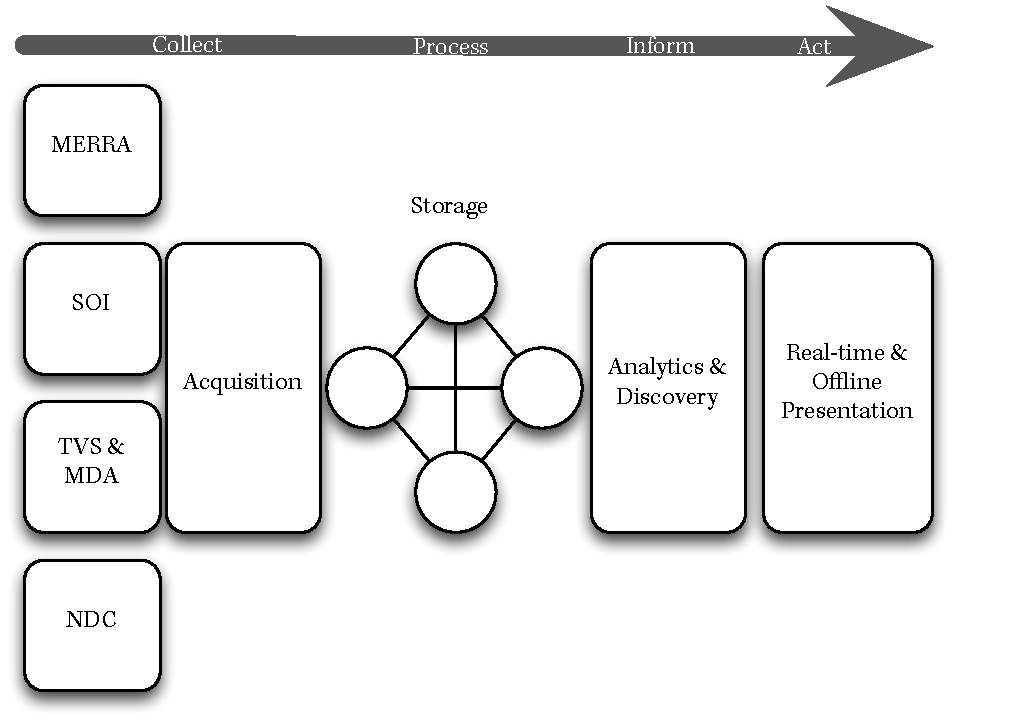
\includegraphics[scale=.9]{dataflow}
\end{figure}

%\begingroup
    % this removes the chapter title for the in-chapter bibliography
%    \renewcommand{\chapter}[2]{}% for other classes
\renewcommand\bibname{{References}}
\bibliographystyle{plain}
\bibliography{chapter2}
%\endgroup
% Review of the sources: internet, C3, books, etc plus interview with the experts

	%!TEX root=index.tex
\chapter{Big Data}

\newacronym{hdf}{HDF}{Hierarchical Data Format}
\newacronym{nosql}{NoSQL}{Not only SQL}


This can be looked at in the first paragaph of the intro


In a guest blog post, Michael Stonebraker gives four detailed definitions to the term big data\index{big data}\cite{stonebraker}. He boils it down to the same basic concepts that most of the non-technical world uses: velocity, volume, or variety. \gls{merra} data is not particularly fast moving by modern measurements: the data can be retrieved in daily (containing hourly measurements) or monthly. As far as volume goes, \gls{merra} is about two hundred terabytes since January 1979 and growing according to Dr. Daniel Walker of CSC[personal communication, 2012]. Lastly, \gls{merra} only comes in as single format known as the \gls{hdf}\cite{hdf}.\\

By Mr. Stonebraker's definition, the most applicable to ClimatEdge\texttrademark{} would be big analytics on big volumes of data. While two hundred terabytes is certainly manageable using commercially available modern hardware, it is too large to fit efficiently on a single system, thus being an excellent candidate for \gls{nosql}\index{noSQL}/big data technologies that tend to scale horizontally (scale out) rather than vertically (scale up).




%\begingroup
    % this removes the chapter title for the in-chapter bibliography
%    \renewcommand{\chapter}[2]{}% for other classes
\renewcommand\bibname{{References}}
\bibliographystyle{plain}
\bibliography{chapter3}
%\endgroup
% Review of the sources: internet, C3, books, etc plus interview with the experts



%\cite{csc_press1}
%Obama’s victory confirmed the value of using technology and data analytics. The technology side of Obama’s campaign was organized into teams to oversee technology, digital and analytics. Engineers working for the campaign developed tools such as Dashboard, an online organizing community, and Obama’s analytics team developed The Optimizer, a tool for placing television advertisements in front of the most optimal audiences for the least amount of money.
%“The Obama campaign proved the power of big data,” says Gary Jackson, CSC’s director of Business Analytics. 
    %!TEX root=index.tex
\chapter{Recommendations}
Recommendations (how should we proceed as a company -- this should Dan's stuff plus the pilot trial for sashi)

In the final two months of 2012, a demonstration was created by a small team of climatologists and engineers for Sashi Reddi, the head of \textsc{CSC's} Big Data and Analytics focus area, to present to the board of directors. This capability demonst




\renewcommand\bibname{{References}}
\bibliographystyle{plain}
\bibliography{chapter4}
    %!TEX root=index.tex
\chapter{Further Research}
\renewcommand\bibname{{References}}
\bibliographystyle{plain}
\bibliography{chapter5}
% Review of the sources: internet, C3, books, etc plus interview with the experts

	%!TEX root=index.tex
\section{Appendix}
\newfontfamily{\anonymous}[Scale=MatchLowercase]{Anonymous Pro}
\lstset{ %
    language=C,                             % Code langugage
    basicstyle=\anonymous,
    tabsize=1,
    breaklines=true,
    breakatwhitespace=false,
    showstringspaces=false,
    showspaces=false,
    showtabs=false
}
Listed below is C code which processes a \gls{merra} data file and stores it within a simple SQLite database \cite{keller1}. Every data type would have a similar parser, typically written in Python for ease of development. However given the complex structure of the \gls{merra} format, combined with the size of the data set, it is reasonable to spend the time to develop it in C to gain execution speed. Processing a single day of \gls{merra} (300MB) and writing into an SQLite flat file takes approximately 20 seconds per variable with the listed code on a modern CPU. Similar code in Python was taking several hours to complete. The entire thirty-three year \gls{merra} archive would take approximately one week to ingest, running in parallel. 
 
\lstinputlisting{/Users/christopher/Documents/work/Climatalytics/prototype/source/merra/c/geo_point.h}
\hrule
\lstinputlisting{/Users/christopher/Documents/work/Climatalytics/prototype/source/merra/c/merra_regex.h}
\hrule
\lstinputlisting{/Users/christopher/Documents/work/Climatalytics/prototype/source/merra/c/merra_regex.c}
\hrule
\lstinputlisting{/Users/christopher/Documents/work/Climatalytics/prototype/source/merra/c/sql.h}
\hrule
\lstinputlisting{/Users/christopher/Documents/work/Climatalytics/prototype/source/merra/c/sql.c}
\hrule
\lstinputlisting{/Users/christopher/Documents/work/Climatalytics/prototype/source/merra/c/latlon.c}
\hrule
\lstinputlisting{/Users/christopher/Documents/work/Climatalytics/prototype/source/merra/c/main.c}
\lstset{ %
    language=Python,                             % Code langugage
    basicstyle=\anonymous,
    tabsize=1,
    breaklines=true,
    breakatwhitespace=false,
    showstringspaces=false,
    showspaces=false,
    showtabs=false
}
A simple mapreduce implementation for word counting in Python is presented below \cite{keller2}.
\lstinputlisting{/Users/christopher/Development/personal/mapreduce_python/pr.py}

    \printglossaries
    \clearpage
    \addcontentsline{toc}{chapter}{Index}
    \printindex
\end{document} 
